\documentclass[11pt]{article}\usepackage[]{graphicx}\usepackage[]{color}
%% maxwidth is the original width if it is less than linewidth
%% otherwise use linewidth (to make sure the graphics do not exceed the margin)
\makeatletter
\def\maxwidth{ %
  \ifdim\Gin@nat@width>\linewidth
    \linewidth
  \else
    \Gin@nat@width
  \fi
}
\makeatother

\definecolor{fgcolor}{rgb}{0.345, 0.345, 0.345}
\newcommand{\hlnum}[1]{\textcolor[rgb]{0.686,0.059,0.569}{#1}}%
\newcommand{\hlstr}[1]{\textcolor[rgb]{0.192,0.494,0.8}{#1}}%
\newcommand{\hlcom}[1]{\textcolor[rgb]{0.678,0.584,0.686}{\textit{#1}}}%
\newcommand{\hlopt}[1]{\textcolor[rgb]{0,0,0}{#1}}%
\newcommand{\hlstd}[1]{\textcolor[rgb]{0.345,0.345,0.345}{#1}}%
\newcommand{\hlkwa}[1]{\textcolor[rgb]{0.161,0.373,0.58}{\textbf{#1}}}%
\newcommand{\hlkwb}[1]{\textcolor[rgb]{0.69,0.353,0.396}{#1}}%
\newcommand{\hlkwc}[1]{\textcolor[rgb]{0.333,0.667,0.333}{#1}}%
\newcommand{\hlkwd}[1]{\textcolor[rgb]{0.737,0.353,0.396}{\textbf{#1}}}%
\let\hlipl\hlkwb

\usepackage{framed}
\makeatletter
\newenvironment{kframe}{%
 \def\at@end@of@kframe{}%
 \ifinner\ifhmode%
  \def\at@end@of@kframe{\end{minipage}}%
  \begin{minipage}{\columnwidth}%
 \fi\fi%
 \def\FrameCommand##1{\hskip\@totalleftmargin \hskip-\fboxsep
 \colorbox{shadecolor}{##1}\hskip-\fboxsep
     % There is no \\@totalrightmargin, so:
     \hskip-\linewidth \hskip-\@totalleftmargin \hskip\columnwidth}%
 \MakeFramed {\advance\hsize-\width
   \@totalleftmargin\z@ \linewidth\hsize
   \@setminipage}}%
 {\par\unskip\endMakeFramed%
 \at@end@of@kframe}
\makeatother

\definecolor{shadecolor}{rgb}{.97, .97, .97}
\definecolor{messagecolor}{rgb}{0, 0, 0}
\definecolor{warningcolor}{rgb}{1, 0, 1}
\definecolor{errorcolor}{rgb}{1, 0, 0}
\newenvironment{knitrout}{}{} % an empty environment to be redefined in TeX

\usepackage{alltt}

\setlength{\oddsidemargin}{0.1in}
\setlength{\textwidth}{6.5in}
\setlength{\topmargin}{-0.5in}
\setlength{\textheight}{9in}
\renewcommand{\baselinestretch}{1.3} 

\usepackage{fancyhdr}
%%\usepackage{fullpage}
%%\usepackage{subfigure}
\usepackage{latexsym}
\usepackage{wrapfig}
\usepackage{graphicx}
\usepackage{pstricks,pst-node,pst-tree,pstricks-add}
\usepackage{amsmath, amsthm, amssymb}
\usepackage{natbib}
\usepackage{algorithm}
\usepackage{algorithmic}
\numberwithin{algorithm}{section}
%%\usepackage{amsfonts}
%\usepackage{nopageno}


%%\usepackage{makeidx}         % allows index generation
%%\usepackage{graphicx}        % standard LaTeX graphics tool
                             % when including figure files
%%\usepackage{multicol}        % used for the two-column index
%%\usepackage[bottom]{footmisc}% places footnotes at page bottom


%% my additional packages 
%%\usepackage{lscape}
%%\usepackage{fancybox}
%%\usepackage{amsfonts,amssymb,amsfonts,amsmath}
%%\usepackage{threeparttable}




%\newcommand{\draftnote}[1]{\marginpar{\tiny\raggedright\textsf{\hspace{0pt}{\bf Comments}:#1}}}
%\newcommand{\draftnote}[1]{}

%%\DeclareMathOperator*{\argmax}{arg\,max}

\newcommand{\cprob}[2]{\ensuremath{\text{Pr}\left(#1 \,|\,#2\right)}}  
\newcommand{\prob}[1]{\ensuremath{\text{Pr}\left(#1 \right)}}
\newcommand{\cexpect}[4]{\ensuremath{\text{E}\left#3 #1 \,|\,#2\right#4}}  
\newcommand{\expect}[3]{\ensuremath{\text{E}\left#2 #1 \right#3}}

\newcommand{\fder}[1]{\frac{d}{d #1}}
\newcommand{\hder}[2]{\frac{d^{#2}}{d {#1}^{#2}}}
\newcommand{\fpart}[1]{\frac{\partial}{\partial #1}}
\newcommand{\hpart}[2]{\frac{\partial^{#2}}{\partial {#1}^{#2}}}
\newcommand{\iid}{\ensuremath{\overset{\text{iid}}{\sim}}}
\newcommand{\indfun}[1]{\ensuremath{1_{\{#1\}}}}
\newcommand{\asarrow}{\ensuremath{\overset{\text{a.s.}}{\rightarrow}}}
\newcommand{\parrow}{\ensuremath{\overset{\text{P}}{\rightarrow}}}
\newcommand{\darrow}{\ensuremath{\overset{\text{D}}{\rightarrow}}}
\newcommand{\mydef}{\ensuremath{\overset{\text{def}}{=}}}

\DeclareMathOperator*{\argmax}{arg\,max}
\DeclareMathOperator*{\argmin}{arg\,min}

\newtheorem*{theorem}{Theorem}
\newtheorem*{prop}{Proposition}
\newtheorem*{corollary}{Corollary}
\newtheorem*{lemma}{Lemma}

\theoremstyle{remark}
\newtheorem*{mynote}{Note}

\theoremstyle{definition}
\newtheorem*{define}{Definition}

\newenvironment{example}[1]{\begin{trivlist}
\item[\hskip \labelsep {\bfseries Example}: \underline{#1}]\ \\}{\end{trivlist}}

\newenvironment{Proof}{\begin{trivlist}
\item[\hskip \labelsep \textit{Proof}:]}{\end{trivlist}}

\newenvironment{exercise}{\begin{trivlist}
\item[\hskip \labelsep \textit{Exercise}:]}{\end{trivlist}}

\newcommand{\todo}[1]{\begin{center}To do: {\bf #1}\end{center}}

%% group numberging of equations and figures by section

%\numberwithin{equation}{section}
%\numberwithin{figure}{section}

\bibliographystyle{plainnat}


\pagestyle{fancy}
\renewcommand{\headrulewidth}{0.8pt}
\lhead{\bf \large SISMID, Module 8 Lecture Notes}
\rhead{\bf Summer 2017}
\chead{} 
\lfoot{} 
\rfoot{} 
\cfoot{\thepage}
%\cfoot{}




%%\usepackage{/Library/Frameworks/R.framework/Resources/share/texmf/Sweave}
\IfFileExists{upquote.sty}{\usepackage{upquote}}{}
\begin{document}

\setkeys{Gin}{width=1.0\textwidth}


\begin{center}
  \textbf{\Large Summer Institute in Statistics and Modeling of Infectious Diseases}\\
  \textbf{\Large Module 8: MCMC Methods for Infectious Disease Studies}\\
  {\large Instructors: Kari Auranen, Elizabeth Halloran and Vladimir Minin}\\
  {\large July 17 -- July 19, 2017}
\end{center}



\section{Probability refresher (self-study material)}


We assume that we can assign probabilities to \textit{events} --- outcomes of a random experiment. For example,
tossing a coin results in one of two possible events: H =``heads" and T=``tails." We also need a concept of a random variable. Informally, a random variable $X$ is a function or variable, whose value is generated by a random experiment. For example, we can define a binary random variable associated with a toss of a coin:
\begin{equation*}
X = 
\begin{cases}
1 &\text{ if heads},\\
0 &\text{ if tails}.
\end{cases}
\end{equation*}

\begin{example}{Discrete uniform random variable}
  Let $X \in \{1,2,\dots,n\}$, with $\prob{X=i} = 1/n$ for all $i = 1,\dots,n$.
\end{example}

\begin{example}{Bernoulli r.v.}
  $X \in \{0,1\}$ with $\prob{X=1}=p$, $\prob{X=0}=1-p$ for $0 \le p \le 1$.
\end{example}

\begin{example}{Binomial r.v.}
  Let $X_i \sim \text{Bernoulli}(p)$. Then the number of successes 
  $S_n = \sum_{i=1}^n X_i$ is called a \textit{binomial r.v.} with 
  \[
  \prob{S_n=k} = {n \choose k} p^k (1-p)^{n-k}.
  \]
\end{example}

\begin{example}{Geometric r.v.}
  $X_1, X_2, \dots$ ordered $\text{Bernoulli}(p)$. Let 
  $N = \min\{n: X_n=1\}$ be the number of trials until the first success occurs, including the 
    the successful trial.
    \[
    \prob{N=n} = (1-p)^{n-1}p  \text{ for } n=1,2,\dots
    \]
\end{example}

\begin{mynote}
  There is an alternative definition of the geometric distribution does not count the successful trial so 
  that $\prob{N=n} = (1-p)^np$.
\end{mynote}

We defined all discrete random variables above using probabilities of $X$ taking a particular value. A function
that assigns probabilities to random variable values is called a \textit{probability mass function}. However, a more
general way to define random variables is by specifying a \underline{cumulative distribution function}.


\begin{define}
  $F(x) = \prob{X \le x}$ is called the \textit{cumulative distribution function} (cdf) of $X$.
\end{define}

\paragraph{Properties of cdf:}
\begin{enumerate}
\item $0 \le F(x) \le 1$.
\item $F(x) \le F(y)$ for $x \le y$.
\item $\lim_{x \rightarrow y^{+}} = F(y)$ ($F(x)$ is right-continuous).
\item $\lim_{x \rightarrow -\infty} = \prob{X=-\infty}$ (usually $=0$)
\item $\lim_{x \rightarrow \infty} = 1-\prob{X=\infty}$ (usually $=1$)
\item $\prob{X=x} = F(x) - F(x^-)$
\end{enumerate}

\begin{example}{Discrete uniform random variable}
  For random variable $U$ uniformly distributed over $\{1,2,\dots,n\}$, its cdf is given by
  \[
  F(x) = 
  \begin{cases}
  0 &\text{ if } x < 1,\\
  \frac{1}{n} &\text { if } 1 \le x < 2,\\
  \frac{2}{n} &\text { if } 2 \le x < 3,\\
  &\vdots\\
  \frac{n-1}{n} &\text { if } n-1 \le x < n,\\
  1 &\text{ if } x \ge n.
  \end{cases} 
  \]
  The probability mass function and cdf of U, with $n=10$, are shown in Figure~\ref{discr-unif-geometric}, which also contains the probability mass function and cdf of a geometric random variable.
\end{example}

\begin{figure}
\centering
\begin{knitrout}
\definecolor{shadecolor}{rgb}{0.969, 0.969, 0.969}\color{fgcolor}

{\centering \includegraphics[width=\maxwidth]{figures/r_discr-pmf-cdf-1} 

}



\end{knitrout}
\caption{Probability mass functions (left column) and cumulative distribution functions (right column) of the discrete uniform 
random variable over $\{1,2,\dots,10\}$ (top row) and geometric random variable with success probability $p = 0.2$ (bottom row).}
\label{discr-unif-geometric}
\end{figure}

For continuous random variables, the analog of the probability mass function is a probability density function,
defined as follows.

\begin{define}
  If $F(x) = \int_{-\infty}^x f(x) dx$ for some $f(x) \ge 0$, then $f(x)$ is called 
  \underline{probability density function} of $X$. If $X$ has a probability density 
  function, we say that $X$ is \underline{absolutely continuous}.
\end{define}

\begin{mynote}
  $\int_a^b f(x) \text{d}x = F(b) - F(a) = \prob{a \le X \le b}$ for $a \le b$. Moreover, 
  $\frac{d}{dx} F(x) = f(x)$. 
\end{mynote}

\begin{example}{Uniform random variable on $[0,1]$}
Random variable $U$ with density 
\[
f(x) = 
\begin{cases}
1 &\text{ if } x \in [0,1],\\
0 &\text{ otherwise}.
\end{cases}
\]
The cdf of $U$ is
\[
F(x) = 
\begin{cases}
0 &\text{ if } x < 0.\\
x &\text{ if } 0 \le x \le 1,\\
1 & \text{ if } x > 1.
\end{cases}
\]
The top row of Figure~\ref{cont-unif-exponential} shows the probability mass function and cdf
of $U$.
\end{example}



\begin{define}
\textit{Expectation} is defined as $E[g(X)] = \int_{-\infty}^{\infty} g(x)dF(x)$, 
where the integral is taken with respect to the measure induced by the cdf, aka probability measure. More concretely,
\begin{enumerate}
\item For discrete random variable $X$, $E[g(X)] = \sum_{k=1}^{\infty} g(x_k) \prob{X=x_k}$.
\item For absolutely continuous random variable $X$, 
$E[g(X)]= \int_{-\infty}^{\infty} g(x) f(x)dx$.
\end{enumerate}
\end{define}

\begin{example}{Exponential r.v.}
  Exponential random variable has density $f(x) = \lambda e^{-\lambda x} \indfun{x \ge 0}$, where $\lambda > 0$
  is the rate parameter. Let $X \sim \text{Exp}(\lambda)$. The probability mass function and 
  cdf of an exponential random variable are shown in the bottom row of Figure~\ref{cont-unif-exponential}.
  Then
  \[
  E(X) = \int_{0}^{\infty}x \lambda e^{-\lambda x} dx =
  \begin{bmatrix}
    u=x & e^{-\lambda x}dx = dv \\
    du=dx & -\frac{e^{-\lambda x}}{\lambda}=v
  \end{bmatrix} =
    \lambda \left[- x \frac{e^{-\lambda x}}{\lambda}  \Big|_{0}^{\infty}  + \int_{0}^{\infty} 
    \frac{e^{-\lambda x}}{\lambda} dx \right]= \lambda \left[0  + \frac{1}{\lambda^2}\right] = \frac{1}{\lambda}.
  \]
\end{example}


Expectations are linear operators, meaning that for any collection of random variables $X_1, \dots, X_n$,
\[
\text{E}\left(\sum_{i=1}^n a_i X_i\right) = \sum_{i=1}^n a_i \text{E}(X_i).
\]
Linearity does not hold for the variance in general. However, if random variables $X_1, \dots, X_n$ are independent, 
then 
\[
\text{Var}\left(\sum_{i=1}^n a_i X_i\right) = \sum_{i=1}^n a_i^2 \text{Var}(X_i).
\]



\begin{figure}
\centering
\begin{knitrout}
\definecolor{shadecolor}{rgb}{0.969, 0.969, 0.969}\color{fgcolor}

{\centering \includegraphics[width=\maxwidth]{figures/r_cont-unif-pmf-cdf-1} 

}



\end{knitrout}
\caption{Probability density functions (left column) and cumulative distribution functions (right column) of the continuous uniform 
random variable on $[0,1]$ (top row) and exponential random variable with rate parameter $\lambda = 2.4$ (bottom row).}
\label{cont-unif-exponential}
\end{figure}



\begin{define}
  For events $A$ and $B$ in $\Omega$ we define \textit{conditional probability} 
  \[
  \cprob{B}{A} = \frac{\prob{A \bigcap B}}{\prob{A}}.
  \]
  If we have a r.v. $X$ defined on $\Omega$, then we can define \textit{conditional expectation}
  \[
  \cexpect{X}{A}{(}{)} = \frac{E(X \indfun{A})}{\prob{A}}.
  \]
\end{define}
Conditioning on random variables is a little tricky, so we'll limit our discussion of this concept to 
\begin{enumerate}
\item discrete case: 
\[
\cprob{X=x}{Y=y} = \frac{\prob{X=x,Y=y}}{\prob{Y=y}},
\]
and
\item absolutely continuous case: 
\[
F_{X\,|\,Y}(x|y) = \frac{\int_{-\infty}^x f_{XY}(z,y)dz}{f_Y(y)} 
\qquad \text{ and } \qquad  
f_{X\,|\,Y}(x|y) = \frac{f_{XY}(x,y)}{f_Y(y)}, 
\]
where $f_{XY}(x,y)$ is the joint density of 
  $X$ and $Y$ and $f_Y(y) = \int_{-\infty}^{\infty} f_{XY}(x,y) dx$ is the marginal density of $Y$.
\end{enumerate}

\begin{define}
  Events $A$ and $B$ are \textit{independent} if $\prob{A \bigcap B} = \prob{A} \prob{B}$. Random variables
  $X$ and $Y$ are called independent if events $\{X \le a\}$ and $\{Y \le b\}$ are independent 
  for all $a,b \in \mathbb{R}$, i.e. $\prob{X \le a, Y \le b} = \prob{X \le a} \prob{Y \le b}$. 
\end{define}

\begin{mynote}
  If r.v.s $X$ and $Y$ are independent, then $\expect{X Y}{(}{)} = \expect{X}{(}{)} \expect{Y}{(}{)}$
  and $\cexpect{X}{Y}{(}{)} = \expect{X}{(}{)}$. The last equality says that $Y$ carries no information 
  about $X$.
\end{mynote}


\begin{example}{Hypergeometric distribution}
  Let $X_1,\dots,X_n \iid \text{Bernoulli}(p)$, $S_n=\sum_{i=1}^n X_i$, and $S_m=\sum_{i=1}^m X_i$ 
  for $m < n$. We want to find the distribution of $S_m$ conditional on $S_n$. We start with 
  probability mass function 
  \[
  \begin{split}
    &\cprob{S_m=j}{S_n=k} = \frac{\prob{S_m=j,S_n=k}}{\prob{S_n=k}} = 
    \frac{\prob{\sum_{i=1}^m X_i=j,\sum_{i=1}^n X_i=k}}{\prob{S_n=k}} \\
    &= \frac{\prob{\sum_{i=1}^m X_i=j,\sum_{i=m+1}^n X_i=k-j}}{\prob{S_n=k}} = [\text{independence}]
    = \frac{\prob{\sum_{i=1}^m X_i=j}\prob{\sum_{i=m+1}^n X_i=k-j}}{\prob{S_n=k}} \\
    &= \frac{\binom{m}{j}p^j(1-p)^{m-j}\binom{n-m}{k-j}p^{k-j}(1-p)^{n-m-k+j}}{\binom{n}{k}p^k(1-p)^{n-k}}
    = \frac{\binom{m}{j}\binom{n-m}{k-j}}{\binom{n}{k}}.
  \end{split}
  \]
  This is the probability mass function of the hypergeometric distribution, which usually is defined 
  as the number of red balls among the $m$ balls drawn from an urn with $k$ red and $n-k$ blue balls.
  \[
  \begin{split}
    &\cexpect{S_m}{S_n=k}{(}{)} = \sum_{i=1}^m \cexpect{X_i}{S_n=k}{(}{)} = [\text{symmetry}] = 
    m \cexpect{X_1}{S_n=k}{(}{)} = \frac{m}{n} \sum_{i=1}^n \cexpect{X_i}{S_n=k}{(}{)}\\ 
    &= \frac{m}{n} \cexpect{S_n}{S_n=k}{(}{)} = \frac{m k}{n}.
  \end{split}
  \]
  Notice that $X_1,\dots,X_n$ don't have to be Bernoulli for $\cexpect{S_m}{S_n}{(}{)} = m S_n /n$ to hold.
\end{example}

\paragraph{Law of total probability}If $B_1,\dots,B_n$ are mutually exclusive events and 
$\bigcup_{i=1}^n B_i = \Omega$, then
\[
\prob{A} = \sum_{i=1}^n \prob{A \bigcap B_i} = \sum_{i=1}^n \cprob{A}{B_i}\prob{B_i}.
\]

\paragraph{Law of total expectation} Recall that $\expect{X}{(}{)}$ is a scalar, but 
$\cexpect{X}{Y}{(}{)}$ is a random variable. Let $X$ and $Y$ be discrete r.v.s. 
\[
\cexpect{X}{Y=y}{(}{)} = \sum_{k=1}^{\infty} x_k \cprob{X=x_k}{Y=y}.
\]
\begin{proof}
\[
\begin{split}
  &\expect{\cexpect{X}{Y}{(}{)}}{[}{]} = \sum_{k=1}^{\infty} \cexpect{X}{Y=y_k}{(}{)} \prob{Y=y_k} =
  \sum_{k=1}^{\infty} \frac{\expect{X \indfun{Y=y_k}}{(}{)}}{\prob{Y=y_k}} \prob{Y=y_k} \\
  &= \sum_{k=1}^{\infty} \expect{X \indfun{Y=y_k}}{(}{)} = 
  \expect{X \indfun{\bigcup_{k=1}^{\infty}\{Y=y_k\}}}{(}{)} = \expect{X}{(}{)}.
\end{split}
\]
\end{proof}
In general, $\expect{\cexpect{X}{Y}{(}{)}}{[}{]} = \expect{X}{(}{)}$. In fact, this equality is often
used as a definition of the conditional expectation, when conditioning on a random variable 
\citep{DurretProbBook}.

\paragraph{Law of total variance} 
Decomposing variance using conditioning is only slightly more complicated:
\[
\begin{split}
&\text{Var}(X) = \expect{X^2}{(}{)} - \expect{X}{(}{)}^2 = [\text{law of total expectation}]
= \expect{\cexpect{X^2}{Y}{(}{)}}{[}{]} - \expect{\cexpect{X}{Y}{(}{)}}{[}{]}^2\\
&=[\text{def of variance}] = \expect{\text{Var}(X \mid Y) + \cexpect{X}{Y}{(}{)}^2}{[}{]} 
- \expect{\cexpect{X}{Y}{(}{)}}{[}{]}^2 = \expect{\text{Var}(X \mid Y)}{[}{]}\\
&+ \left\{\expect{\cexpect{X}{Y}{(}{)}^2}{[}{]} - \expect{\cexpect{X}{Y}{(}{)}}{[}{]}^2\right\}
= [\text{def of variance}] = \text{E}\left[\text{Var}(X \mid Y)\right] + \text{Var}\left[\text{E}(X \mid Y)\right].
\end{split}
\]

Later in the course, we will be using the following two limit theorems that describe asymptotic behavior of empirical averages of random variables.

\begin{theorem}{Strong Law of Large Numbers (SLLN).}
Let $X_1, X_2, \dots$ be independent and identically distributed (iid) random variables
with $\mu = \text{E}(X_1) < \infty$. Then
\[
\lim_{n \rightarrow \infty} \frac{1}{n}\sum_{i=1}^n X_i = \mu.
\]
\end{theorem}
SLLN says that the empirical average of iid random variables converges to the theoretical average/expectation.

\begin{theorem}{Central Limit Theorem (CLT).}
Let $X_1,X_2,\dots$ be independent and identically distributed (iid) random variables
with $\mu = \text{E}(X_1) < \infty$ and $0 < \sigma^2 = \text{Var}(X_1)  < \infty$ and let $\bar{X}_n = (1/n)\sum_{i=1}^n X_i$. Then
\[
\frac{\sqrt{n}(\bar{X}_n - \mu)}{\sigma} \sim \mathcal{N}(0,1) \text{ approximately for large } n.
\]
\end{theorem}
Informally, CLT says that for large $n$, the empirical average behaves as $\mathcal{N}(\mu, \sigma^2/n)$. Scaling of the variance by $1/n$ implies that averaging reduces
variability, which makes intuitive sense. 

\clearpage

\section{Monte Carlo methods}
The rest of the notes are largely based on \citep{RobertANDCasella}. Although our driving applications of 
Monte Carlo integration will mostly revolve around Bayesian inference, we would like to point out that
all Monte Carlo methods can (should?) be viewed as a numerical integration problem. 
Such problems usually start with either discrete ($\mathbf{x}$) or continuous ($\boldsymbol{\theta}$) 
vector of random variables. Despite the fact that distributions of these vectors are known only 
up to a proportionality constant, we are interested in taking expectations with respect to these distributions.
Compare the following integration problems faced by physicists and Bayesian statisticians.
\begin{center}
  \begin{tabular*}{0.9\textwidth}{@{\extracolsep{\fill}}cc}
    \textit{Statistical mechanics} & \textit{Bayesian statistics} \\  
      $\displaystyle \prob{\mathbf{x}} = \frac{1}{Z} e^{-\mathcal{E}(\mathbf{x})}$ &
      $\displaystyle \cprob{\boldsymbol{\theta}}{\mathbf{y}} = \frac{1}{C} \cprob{\mathbf{y}}{\boldsymbol{\theta}}
      \prob{\boldsymbol{\theta}}$ \\
      Objective: $\text{E}[f(\mathbf{x})] = \sum_{\mathbf{x}} f(\mathbf{x})\prob{\mathbf{x}}$ &
      Objective: $\text{E}[f(\mathbf{\boldsymbol{\theta}})\,|\,\mathbf{y}] = 
      \int f(\boldsymbol{\theta})\cprob{\boldsymbol{\theta}}{\mathbf{y}}\text{d}\boldsymbol{\theta}$
  \end{tabular*}
\end{center}
\begin{mynote}
  Many applications involve both, intractable summation and integration:
  \begin{equation*}
    \text{E}[f(\mathbf{x},\boldsymbol{\theta})] = 
    \sum_{\mathbf{x}}\int f(\boldsymbol{\mathbf{x},\theta})\prob{\mathbf{x},\boldsymbol{\theta}}
    \text{d}\boldsymbol{\theta}.
  \end{equation*}
\end{mynote}
The above integration problems are difficult to solve even numerically, especially in high dimensions,
e.g. when the length of $\mathbf{x}$ and/or $\boldsymbol{\theta}$ is on the order of $10^3-10^6$.
All Monte Carlo techniques attempt to solve such high dimensional integration problems by stochastic 
simulation. 
%To execute such stochastic simulations, we first need to know how to generate
%random variables in one dimension.


\subsection{Classical Monte Carlo}
In general, Monte Carlo integration aims at approximating expectations 
of the form
\begin{equation}
  \text{E}[h(X)] = \int h(x) f(x) \text{d}x.
  \label{gen-int}
\end{equation}
If $X_1,...,X_n {\buildrel \text{iid} \over \sim} f(x)$ and $\text{E}[h(X_1)] < \infty$ , 
then we know from the strong law of large number (SLLN) that 
\begin{equation*}
  \frac{1}{n} \sum_{i =
    1}^ n h(X_i) {\buildrel \text{a.s.} \over \rightarrow} \text{E}_f[h(X_1)].
\end{equation*}
Therefore, we can approximate the desired expectation with 
\begin{equation*}
  \bar{h}_n = \frac{1}{n} \sum_{i=1}^ n h(X_i) \approx \text{E}_f[h(X_1)]
\end{equation*}
for some large, yet finite $n$. Conveniently, the variance of this Monte Carlo estimator can be approximated
as 
\begin{equation*}
  \text{Var}(\bar{h}_n) = \frac{1}{n^2} \times n \times \text{Var}[h(X_1)] = 
  \frac{1}{n} \int \left\{h(x) - \text{E}_{f}[h(x)]\right\}^2 f(x) \text{d}x 
  \approx \frac{1}{n^2} \sum_{i=1}^n \left[h(X_i) - \bar{h}_n\right]^2 = v_n
\end{equation*}
Moreover, the central limit theorem says that
\begin{equation*}
  \frac{\bar{h}_n - \text{E}_f[h(X_1)]}{\sqrt{v_n}} 
  {\buildrel \text{D} \over \rightarrow}  \mathcal{N}(0,1),
\end{equation*}
allowing us to estimate the Monte Carlo error, e.g. $\bar{h}_n \pm 1.96 \sqrt{v_n}$.

\subsection*{Importance Sampling}
In many situations classical Monte Carlo is impossible, because we can not sample from the target
distribution $f(x)$. Therefore, we would like to be able to compute the integral (\ref{gen-int})
by sampling from some other, perhaps simpler, distribution $g(x)$. Importance sampling allows us to 
accomplish this task. The main idea is to rewrite the expectation of interest as
\begin{equation*}
  \text{E}_f[h(X)]=  
  \int h(x)\frac{f(x)}{g(x)}g(x)\text{d}x = \text{E}_g\left[h(X) \frac{f(X)}{g(X)}\right].  
\end{equation*}
This representation suggests that we can generate $X_1,...,X_n {\buildrel \text{iid} \over \sim} g(x)$ and 
use the SLLN again to arrive at the approximation
\begin{equation*}
  \text{E}_f[h(X)] \approx \frac{1}{n}\sum_{i = 1}^n \frac{f(X_i)}{g(X_i)}h(X_i).
\end{equation*}
Notice that the above approximation still requires knowledge of the normalizing constant of $f(x)$, which
is unrealistic in most applications of importance sampling. Luckily there is an alternative importance
sampling estimator that is as easy to compute as the original one:
\begin{equation*}
  \text{E}_f[h(X)] \approx  \frac{\sum_{i=1}^n h(X_i) \frac{f(X_i)}{g(X_i)}}{\sum_{i=1}^n \frac{f(X_i)}{g(X_i)}}.  
\end{equation*}
In this estimator, the normalizing constants of both $f(x)$ and $g(x)$ cancel out and the denominator
converges to $\int \frac{f(x)}{g(x)}g(x) \text{d}x = \int f(x)\text{d}x = 1$ by the SLLN again.
\par
As illustrated by the next example, the importance sampling can be useful even if we can easily 
simulate from $f(x)$, because importance sampling can be used to reduce the Monte Carlo variance.

In conclusion, we point out that the most difficult aspect of classical Monte Carlo is generating
iid samples. Even importance sampling has severe limitations in high dimensions. In such difficult 
cases, Markov chain Monte Carlo (MCMC) can come to rescue. Before we master this numerical integration
technique we need to refresh our knowledge of Markov chains.

\begin{example}{Estimating the tail of the standard normal distribution}
See practical in `dtmc-lab.pdf'.
\end{example}

\subsection{Elementary Markov chain theory}
In this section we will cover some basic results for Markov chains. For a more detailed treatment, see for example
\citep{BremaudBook}.

\subsubsection{Definitions and examples}

\begin{define}
A \underline{stochastic process} is a family of ordered random variables $X_t$, where $t$
ranges over a suitable index set $T$, e.g. $T_1 = [0, \infty)$, $T_2 =
\{1,2,...\}$.
\end{define}

\begin{define}
  A discrete time stochastic process $\{X_n\}_{n=0}^\infty$ is
  called a \underline{Markov chain} if for all $n \ge 0$ and for all 
  $i_0, i_1, ..., i_{n-1}, i, j$,
  \begin{equation*}
    \text{P}(X_{n+1} = j\,|\, X_n = i, X_{n-1} = i_{n-1}, ..., X_0 = i_0) = 
    \text{P}(X_{n + 1} = j \,|\, X_n = i).
  \end{equation*}

\noindent
We call $X_n$ a \underline{homogeneous Markov chain} if $\cprob{X_{n+1} = j}{X_n = i}$ 
is independent of $n$, and \underline{inhomogeneous} otherwise.
We also define \underline{1-step transition probabilities}
\begin{equation*}
  p_{ij} = \cprob{X_1 = j }{X_0 = i} \quad \sum_j p_{ij} = 1, p_{ij} \ge 0 \text{ for all } i,j
\end{equation*}
and \underline{n-step transition probabilities}
\begin{equation*}
  p_{ij}^{(n)} = \cprob{X_{n} = j}{X_0 = i}, \quad \sum_j p_{ij}^{(n)} = 1, 
  p_{ij}^{(n)} \ge 0 \text{ for all } i,j
\end{equation*}
and collect them into \underline{transition probability matrix} $\mathbf{P} = \{p_{ij}\}$
and \underline{n-step transition probability matrix} $\mathbf{P}^{(n)} = \{p_{ij}^{(n)}\}$.
\end{define}

\begin{mynote}
  A Markov chained is fully specified by its transition probability matrix $\mathbf{P}$ 
  and an initial distribution $\boldsymbol{\nu}$.
\end{mynote}

\begin{mynote}
  It is easy to show that $n$-step transition probabilities can be obtained by repeatedly multiplying
  transition probability matrix by itself. More precisely, $\mathbf{P}^{(n)} = \mathbf{P}^n$. This observation
  makes it easy to compute the marginal distribution of $X_n$, 
  $\boldsymbol{\nu}^{(n)} = (\nu_1^{(n)},\dots,\nu_s^{(n)})$, 
  where $ \nu_i^{(n)} = \text{Pr}(X_n = i)$. Then  
  \begin{equation*}
    \boldsymbol{\nu}^{(n)} = \boldsymbol{\nu} \mathbf{P}^n.
  \end{equation*}
\end{mynote}

\begin{define}
  A Markov chain with transition probability matrix $\mathbf{P}$ is called \underline{irreducible} if 
  for any pair of states $(i,j)$ there exists $n > 0$ such that $p_{ij}^{(n)} > 0$ and 
  \underline{reducible} otherwise. In other words,
  an irreducible Markov chain can get from any state to any state in a finite number of steps with 
  positive provability.
\end{define}

\begin{example}{SIS model}
Suppose we observe an individual over a sequence of days $n=1,2,\dots$ and classify this individual each
day as
\begin{equation*}
  X_n = \begin{cases}
    I &\text{if infected}\\
    S &\text{if susceptible}.
  \end{cases}
\end{equation*}
  \begin{center}

  \end{center}
We would like to construct a stochastic model for the sequence $\{X_n\}_{n=1}^{\infty}$. 
One possibility is to assume that $X_n$s are independent and
$\text{P}(X_n=I) = 1-\text{P}(X_n=S)=p$. However, this model is not very realistic
since we know from experience that the individual is more likely to stay infected if he or she
is already infected.  Since Markov chains are the simplest models that allow us to relax independence, 
we proceed by defining a transition probability matrix
\begin{minipage}[c]{0.5\textwidth}
  \begin{equation*}
    \mathbf{P} = \begin{pmatrix}
      1-p & p\\
      q & 1-q
    \end{pmatrix}
  \end{equation*}
\end{minipage}
\begin{minipage}[r]{0.4\textwidth}
  %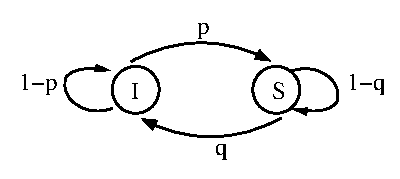
\includegraphics{sis}
\end{minipage}

The directed graph with labeled edges, shown next to the matrix, graphically encodes
the same information contained in the transition probability matrix. Such graphs are called 
transition graphs of Markov chains. If $p$ and $q$ are strictly positive, then the Markov chain
is irreducible.
\end{example}

\subsubsection{Stationary distribution and long term behavior}

\begin{define}
  Any probability distribution $\boldsymbol{\pi}$ on state space $E$ that
  satisfies $\boldsymbol{\pi}^T = \boldsymbol{\pi}^T\mathbf{P}$ (also called the global balance
  equation) is called a \underline{stationary (or equilibrium) distribution} of the
  corresponding homogeneous Markov chain.  
\end{define}

\begin{mynote}
  $\boldsymbol{\pi}^T = \boldsymbol{\pi}^T P$ if and only if $\pi(i) = \sum_{j \in E} \pi_jp_{ji}$ for all $i \in E$.
\end{mynote}


\begin{example}{SIS model continued}
  Let's assume that $0 < p < 1$ and $0 < q < 1$ in the SIS model. Then global equations become
  \begin{equation*}
    (\pi_1, \pi_2) 
    \begin{pmatrix}
      1-p & p \\
      q &1-q
    \end{pmatrix}=
    (\pi_1,\pi_2) 
    \Rightarrow
  \begin{cases}
    \pi_1(1-p) + \pi_2 q &= \pi_1\\
    \pi_1 p + (1-q)\pi_2 &= \pi_2
  \end{cases}
  \Rightarrow \pi_1 = \frac{q}{p} \pi_2.
  \end{equation*} 
\end{example}
Adding the constraint $\pi_1 + \pi_2 = 1$, we obtain the unique solution 
\begin{equation*}
  \pi_1 = \frac{q}{p+q} \qquad \text{ and } \qquad \pi_2 = \frac{p}{p+q}.
\end{equation*}

Not all Markov chains have a stationary distribution and if a stationary distribution exists, it may be
not unique as illustrated by the following example.

%%\begin{example}{SIR model}
%%The set up is similar to the SIS model, except we assume that infected individuals have a positive 
%%probability of developing immunity to the disease. We call such individuals removed from the population 
%%of interest. The transition matrix and the corresponding Markov chain graph become
%%\begin{equation*}
%%  \mathbf{P} = \begin{pmatrix}
%%    1-p & p & 0\\
%%    q & r & (1-r-q)\\
%%    0 & 0 & 1
%%  \end{pmatrix} \qquad \qquad \qquad \qquad
%%\psmatrix[colsep=2.5cm,rowsep=1.5cm,mnode=circle]
%%\psset{arrowscale=2,linewidth=10pt}
%%\text{\Large S}&\text{\Large I}&\text{\Large R}
%%\ncarc[arcangle=40]{->}{1,1}{1,2}^{p}
%%\ncarc[arcangle=40]{->}{1,2}{1,1}_{q}
%%\ncarc[arcangle=40]{->}{1,2}{1,3}^{1-r-q}
%%\nccircle[angleA=90]{->}{1,1}{.4cm}<{1-p}
%%\nccircle[angleA=-140]{->}{1,2}{.4cm}>{r}
%%\nccircle[angleA=-90]{->}{1,3}{.4cm}>{1.}
%%\endpsmatrix
%%\end{equation*}
%%\end{example}

\begin{example}{Gambler's ruin}
In this example, we assume that a gambler can increase or decrease his/her fortune by one with 
corresponding probabilities $p$ and $q=1-p$. The game ends as soon the gambler runs out of money or
reaches a predefined fortune, 4 in our example. The transition matrix and the corresponding transition 
graph are shown below.
\begin{equation*}
  \begin{pmatrix}
    1 & 0 & 0 & 0 & 0 \\
    q & 0 & p & 0 & 0 \\
    0 & q & 0 & p & 0 \\
    0 & 0 & q & 0 & p \\
    0 & 0 & 0 & 0 & 1
  \end{pmatrix}\qquad \qquad \qquad
  \psmatrix[colsep=1.5cm,rowsep=1.5cm,mnode=circle]
  \psset{arrowscale=2,linewidth=10pt}
  \text{\Large 0}& \text{\Large 1}&\text{\Large 2}&\text{\Large 3}&\text{\Large 4}
  \ncarc[arcangle=40]{->}{1,2}{1,3}^{p}
  \ncarc[arcangle=40]{->}{1,3}{1,4}^{p}
  \ncarc[arcangle=40]{->}{1,4}{1,5}^{p}
  \ncarc[arcangle=40]{->}{1,2}{1,1}_{q}
  \ncarc[arcangle=40]{->}{1,3}{1,2}_{q}
  \ncarc[arcangle=40]{->}{1,4}{1,3}_{q}
  \nccircle[angleA=90]{->}{1,1}{.4cm}<{1}
  \nccircle[angleA=-90]{->}{1,5}{.4cm}>{1.}
  \endpsmatrix
\end{equation*}
The chain is reducible, because it is impossible to get out of states 0 and 4. Such states are called
\underline{absorbing states}.
It is easy to show that vector $\boldsymbol{\pi}^{T} =(\alpha,0,0,0,1-\alpha)$ satisfies 
$\boldsymbol{\pi}^{T}\mathbf{P} = \boldsymbol{\pi}$ for any $\alpha \in [0,1]$.
\par 
\end{example}

%%\begin{exercise}
%%  For $p=0.4$ and each starting state $i=1,2,3$, 
%%  estimate the mean time to absorption, $T(i)$, for the gambler's ruin 
%%  example via classical Monte Carlo. 
%%\end{exercise}

Global balance equations can be hard to check in practice when the Markov chain state space is large. 
However, there is an easier set of equations that one can check to ensure that a stationary distribution
exists.

\begin{define}
  A probability vector $\boldsymbol{\pi}$ is said to satisfy 
  \underline{detailed balance equations} with respect to stochastic matrix $\mathbf{P}$ if 
  \begin{equation*}
    \pi_i p_{ij} = \pi_j p_{ji} \text{ for all } i,j.
  \end{equation*}
\end{define}

\begin{prop}(detail balance $\Rightarrow$ global balance)
  Let $\mathbf{P}$ be a transition probability matrix of $X_n$ on $E$ and let $\boldsymbol{\pi}$ be a
probability distribution on $E$. If $\boldsymbol{\pi}$ satisfies detailed balance equations, then 
$\boldsymbol{\pi}$ also satisfies global balance equations.
\end{prop}

\begin{Proof}
  $\pi_i p_{ij} = \pi_j p_{ji}
  \Rightarrow \sum_{j \in E} \pi_ip_{ij} 
  = \pi_i\cdot 1 
  = \sum_{j\in E} \pi_j p_{ji}. \qed$
\end{Proof}
\begin{mynote}
  Markov chains with a stationary distribution that satisfies detailed balance equations are often 
  called \underline{reversible Markov chains}. However, there is some disagreement among textbook
  authors about this term. For example, some authors require reversible chains to have initial
  distribution being equal to the stationary distribution. Irreducibility is also often added to 
  the list of requirements for reversible Markov chains.
\end{mynote}

\begin{example}{Ehrenfest model of diffusion}
Imagine a two dimensional rectangular box with a divider in the middle. The box contains $N$ balls
(gas molecules)  distributed somehow between the two halves. The divider has a small gap, through which 
balls can go through one at a time. We assume that at each time step we select a ball uniformly at 
random and force it go through the gap to the opposite side of the divider. Letting $X_n$ denote
the total number of balls in the left half of the box, our Markov process is described by the 
following transition probabilities.

\begin{minipage}[c]{0.5\textwidth}
  \[
  p_{ij} =
  \begin{cases}
    \frac{i}{N}. &\text{ for } j=i-1,\\\
    1-\frac{i}{N}, &\text{ for } j=i+1,\\
    0, \text{ otherwise}.
  \end{cases}
  \]
\end{minipage}
\begin{minipage}[r]{0.45\textwidth}
  \vspace{0.2cm}
  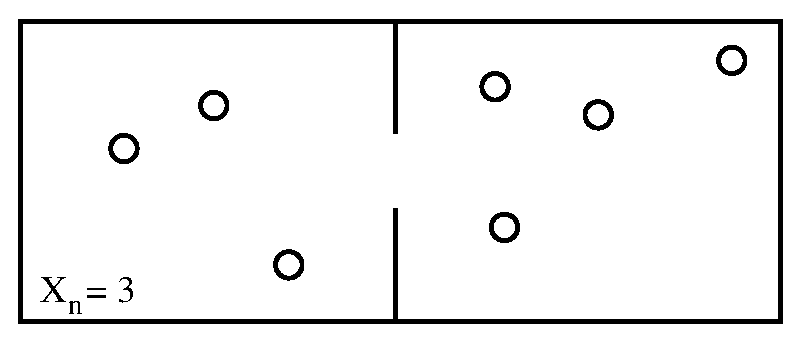
\includegraphics[width=0.9\textwidth]{ehrenfest}
  \vspace{0.3cm}
\end{minipage}

If we want to derive a stationary distribution of the system, we can solve the global balance equations
$\boldsymbol{\pi}^T \mathbf{P} = \boldsymbol{\pi}^{T}$. Alternatively, we may ``guess'' that at
equilibrium $X_n \sim \text{bin}(\frac{1}{2}, N)$ and verify this candidate stationary distribution
via detailed balance. Notice we do not know whether the Ehrenfest chain is reversible, but we'll go
ahead with the detailed balance check anyway. First, notice that entries of our candidate vector are
\begin{equation*}
  \pi_i = {N \choose i} \left(\frac{1}{2}\right)^i\left(1-\frac{1}{2}\right)^{N-i} = 
  {N \choose i} \frac{1}{2^N}
\end{equation*}
Since $X_n$ can only increase or decrease by one at each time step, we need to check detailed balance 
only for $i$ and $j = i + 1$.  
\[
\begin{split}
  &\pi_i p_{i,i+1} = \frac{1}{2^N}{N \choose i} \frac{N - i}{N} =
  \frac{1}{2^N} \frac{N!}{i!(N-i)!} \frac{N - i}{N} =
  \frac{1}{2^N} \frac{N!}{(i+1)!(N-i-1)!} \frac{i+1}{N}\\
  &= {N \choose i+1} \frac{1}{2^N} \frac{i+1}{N} = \pi_{i+1} p_{i+1,i},
\end{split}
\]
confirming our guess.
\end{example}

\begin{define}
  An irreducible Markov chain is called \underline{recurrent} if starting from any state the chain 
  returns this state eventually with probability one. The recurrent chain is called 
  \underline{positive recurrent} if all expected return times are finite.
\end{define}

\begin{prop}
  If a Markov chain is irreducible and positive recurrent, then there exists a stationary distribution and 
  this distribution is unique.
\end{prop}

\begin{mynote}
  Irreducible Markov chains on finite state spaces are always positive recurrent.
\end{mynote}

\begin{prop}
  An irreducible Markov chain is positive recurrent if and only if the chain possesses a stationary distribution.
\end{prop}

\begin{theorem}{(Ergodic Theorem)}
  Let $\{X_n\}$ be an irreducible positive recurrent Markov chain with stationary distribution 
  $\boldsymbol{\pi}$ and let $f: E \rightarrow \mathbb{R}$ be an arbitrary function that maps Markov chain
  states to real numbers satisfying $\sum_{i \in E} |f(i)| \pi_i < \infty$. Then for any initial distribution
  \begin{equation*}
    \lim_{N \rightarrow \infty}\underbrace{\frac{1}{N}\sum_{k=1}^N f(X_k)}_{\text{time average}} 
    = \sum_{i \in E} f(i) \pi_i = \underbrace{\text{E}_{\boldsymbol{\pi}}[f(X)]}_{\text{space average}}.
  \end{equation*}
\end{theorem}

\begin{example}{Ehrenfest model of diffusion (continued)}
Separate practical.
\end{example}

\begin{mynote}
  Just as the strong law of large numbers is the key behind Monte Carlo
  simulations, the ergodic theorem for Markov Chains is the reason why Markov chain Monte Carlo (MCMC) works.
  This remark naturally leads us to the next section.
\end{mynote}


\subsection{Markov chain Monte Carlo}
Before we dive into MCMC, let's ask ourselves why we are not happy with classical Monte Carlo and if there is 
any need to invent something more complicated. The main motivation for developing MCMC is the fact 
that classical Monte Carlo is very hard to implement in high dimensional spaces. MCMC also often 
experiences difficulties in high dimensions. However, for almost any high dimensional integration, it is fairly
straightforward to formulate an MCMC algorithm, while the same is not true for classical Monte Carlo.
\par
Recall that our objective in MCMC is the same as in classical Monte Carlo: to estimate expectations of 
the form
\begin{equation*}
  \text{E}_{\boldsymbol{\pi}}[h(\mathbf{x})] = \sum_{\boldsymbol{x} \in E} \pi_{\boldsymbol{x}} h(\mathbf{x}).
\end{equation*}
Notice that here we assume that our state space is discrete so the above expectation is a finite sum.
However we assume that the size of $E$ is so large that carrying out this summation even on fastest computers
is impractical. We also assume that we do not know how to produce iid samples from $\boldsymbol{\pi}$.
The general MCMC strategy then is to construct an ergodic Markov chain $\{X_n\}$
with stationary distribution $\boldsymbol{\pi}$. Then from the ergodic theorem and $N$ realizations from
the Markov chain, we get
\begin{equation*}
  \text{E}_{\boldsymbol{\pi}}[h(\mathbf{x})] \approx \frac{1}{N} \sum_{i = 1}^N h(X_i).
\end{equation*}
The question is how to construct such a Markov chain, $\{X_n\}$.


\subsubsection{Metropolis-Hastings algorithm}
As always in MCMC, we start with a target distribution $\boldsymbol{\pi}$. 
Given some initial value $X_0 = x_0$, we construct a Markov chain according to the following set of rules \citep{Hastings1970}.
\begin{algorithm}
\caption{Metropolis-Hastings Algorithm: approximate $\text{E}_{\boldsymbol{\pi}}[h(\mathbf{x})]$}
\label{accept-reject}
\begin{algorithmic}[1]
  \STATE Start with some initial value $X_0 = x_0$.
  \FOR{$n=0$ to $N$}
  \STATE Simulate a candidate value $Y \sim q(j\,|\,X_n=i)$. Suppose $Y=j$.
  \STATE Compute the Metropolis-Hastings \underline{acceptance probability}
  \begin{equation*}
    a_{ij} = \min \left\{ \frac{\pi_j q(i\,|\, j)}{\pi_i q(j\,|\, i)}, 1 \right\}
  \end{equation*}
  \STATE Generate $U \sim \text{Unif}[0,1]$.  
  \STATE Accept the candidate $Y=j$ if $U \le a_{ij}$, otherwise set $X_{n+1} = X_n$. 
  More specifically, set
  \begin{equation*}
    X_{n+1} = \begin{cases} 
       Y & \text{ if } U \le a_{ij} \\
       X_n & \text{ if } U > a_{ij} 
     \end{cases} 
 \end{equation*}
\ENDFOR
\RETURN $\frac{1}{N} \sum_{i = 1}^N h(X_i)$.
\end{algorithmic}
\end{algorithm}

\begin{prop} 
  The Metropolis-Hastings algorithm generates a Markov chain with stationary distribution 
  $\boldsymbol{\pi}$.
\end{prop}

\begin{Proof}
Let $\mathbf{P} = \{p_{ij}\}$ be the transition matrix for $X_n$. Then for $i \ne j$,
\begin{equation*}
  p_{ij} = \text{Pr}(X_{n+1} = j \,|\, X_n = i) =  \text{Pr}(X_1 = j \,|\, X_0 = i)
  = a_{ij} q(j\,|\,i).
\end{equation*}
Again, for $i \ne j$,
\begin{equation*}
  \pi_i p_{ij} = \pi_i a_{ij} q(j \,|\, i) = 
  \begin{cases}
    \pi_i q(j \,|\, i) \dfrac{\pi_j q(i \,|\, j)}{\pi_i q(j \,|\, i)} & \text{ if }
    \dfrac{\pi_j q(i \,|\, j)}{\pi_i q(j \,|\, i)} \le 1 \\
    \pi_i q(j \,|\, i) \cdot 1 & \text{ otherwise }
  \end{cases} \\
  = 
  \begin{cases}
    \pi_j q(i \,|\, j) & \text{ if }
    \dfrac{\pi_j q(i \,|\, j)}{\pi_i q(j \,|\, i)} \le 1 \\
    \pi_i q(j \,|\, i) & \text{ otherwise }
  \end{cases}
\end{equation*}
and
\begin{equation*}
  \pi_j p_{ji} = \pi_j a_{ji} q(i\,|\, j) = \begin{cases}
    \pi_j q(i\,|\, j) \cdot 1
    & \text{ if }
    \dfrac{\pi_j q(i\,|\, j)}{\pi_i q(j\,|\, i)} \le 1 \\
    \pi_j q(i\,|\, j) \dfrac{\pi_i q(j\,|\, i)}{\pi_j q(i\,|\, j)}  &
    \text{ otherwise }
  \end{cases}
  = \begin{cases}
    \pi_j q(i \,|\, j) &
    \text{ if } \dfrac{\pi_j q(i \,|\, j)}{\pi_i q(j \,|\, i)} \le 1 \\
    \pi_i q(j \,|\, i) &
    \text{ otherwise }
  \end{cases}
\end{equation*}
So we have shown $\pi_i p_{ij} = \pi_j p_{ji}$. We require $\pi_i > 0$ for all $i$ and 
$q(i |j) > 0 \Leftrightarrow q(j|i) > 0$.  Since we have detailed balance, we conclude that 
$\boldsymbol{\pi}$ is a stationary distribution.$\qed$
\end{Proof}

\begin{mynote}
  If we choose $\{q(i,j)\}$ so that $\{X_n\}$ is irreducible, then $\{X_n\}$
  is positive recurrent by the stationary distribution criterion.
  Therefore, we can use the Ergodic theorem.
\end{mynote}

\begin{mynote}
  We do not need a normalizing constant of $\boldsymbol{\pi}$ in order to
  execute the Metropolis-Hastings algorithm. This is important, because in most applications of MCMC (e.g., Bayesian statistics)
  the target distribution is not normalized and the normalization constant is unknown. 
\end{mynote}

\begin{example}{Toric Ising model on a circle}
  We model ferromagnetism with a set of $n$ electron spins, $\mathbf{x}$. We assume that spins are arranged on 
  a circles and have two directions, denoted by $1$ and $-1$. The Gibbs distribution of configuration $\mathbf{x}$
  is 
  \[
  \pi(\mathbf{x}) = \frac{1}{Z} e^{\beta \sum_{i=1}^n x_i x_{i+1}}, 
  \]
  where the normalizing constant 
  \[
  Z = \sum_{\mathbf{x} \in \{1,-1\}^n} e^{\beta \sum_{i=1}^n x_i x_{i+1}}
  \]
  is called a partition function. In this particular example, $Z$ can be computed using a transfer matrix method,
  but we will pretend that $Z$ is not available to us. 
  \par
  To set up a Metropolis-Hastings algorithm, we need a proposal mechanism to move from one configuration to 
  another. At each step, let's choose a site uniformly at random and change the direction of the spin. This 
  translates to the proposal probabilities
  \[
  q(\mathbf{y}\,|\,\mathbf{x}) =   q(\mathbf{x}\,|\,\mathbf{y}) = 
  \begin{cases}
    \frac{1}{n} &\text{ if } \mathbf{x} \text{ and } \mathbf{y} \text{ differ at exactly one location},\\
    0 & \text{ otherwise}.
  \end{cases}
  \]
  If $\mathbf{x}^{(t)}$ is the current state of the Markov chain and $\mathbf{x}'$ is a proposed state with 
  the $j$th site changed to the opposite direction, then 
  \[
  a_{\mathbf{x}^{(t)}, \mathbf{x}'} = \frac{\pi(\mathbf{x}')\frac{1}{n}}{\pi(\mathbf{x}^{(t)})\frac{1}{n}} = 
  \frac{e^{\beta \sum_{i \notin \{j,j-1\}} x_i^{(t)}x_{i+1}^{(t)}} e^{\beta (-x_{j-1}^{(t)}x_j^{(t)} -x_{j}^{(t)}x_{j+1}^{(t)})}}
  {e^{\beta \sum_{i \notin \{j,j-1\}} x_i^{(t)}x_{i+1}^{(t)}} e^{\beta (x_{j-1}^{(t)}x_j^{(t)} + x_{j}^{(t)}x_{j+1}^{(t)})}} = 
  e^{-2 \beta x_j^{(t)}(x_{j-1}^{(t)}+x_{j+1}^{(t)})}.
  \]
  Clearly, this proposal mechanism makes it possible to get from any state to any other state of spin 
  configurations, so the Metropolis-Hastings chain is irreducible.
\end{example}


Variants of Metropolis-Hastings:
\begin{enumerate}
 \item $q(i\,|\, j) = q(j\,|\, i)$ - symmetric proposal.  This is the
   original Metropolis algorithm \citep{Metropolis1953}.  Here, the acceptance probability
   simplifies to $a_{ij} = \min\left\{ \frac{\pi_j}{\pi_i}, 1 \right\}$.
   So we move to a more probable state with probability 1, and move
   to less probable states sometimes (more rarely if the candidate
   is much less probable).

 \item Independence sampler: $q(j\,|\,i) = q(j)$.  Note this
   is \emph{not} the same as iid sampling.  Independence sampler is still a Markov chain,
   since the sampler can stay in the same place with some probability at each step of 
   the algorithm.
\end{enumerate}

% \subsubsection{Markov chains on continuous state spaces}

% \bdf
% A sequence of random variables $\{X_n\}$ is a \emph{Markov chain in a
% continuous state space $E$} if for all $t$ and for all $A \subset E$, we
% have
% \EAL{
% \Pof{X_{n+1} \in A \C X_n, X_{n-1}, \ldots, X_0} &= \Pof{X_{n+1} \C X_n} \\
% &=  \Pof{X_1 \C X_0}  \qquad\text{(homogeneity)}
% }

% We call $K(X,A) \eqdef \Pof{X_1 \in A \C X_0}$ the \emph{transition
% kernel}, and if we have a conditional density $f(y \C X)$ such that
% \EQl{ K(X,A) = \Pof{X_1 \in A \C X_0} = \int_A f(y \C X) dy }
% then we call $f(y \C X)$ the \emph{transition kernel density}.
% \edf

% \bthmn{Chapman-Kolmogorov}
% \EQl{ K^{m+n}(X,A) = \int_E K^n(y,A) \underbrace{K^m(X,dy)}_{\stackrel{=
% f(y \C X)}{\text{ if you have a density}}} }
% \ethm

% \bdf A \emph{stationary distribution} is a measure $\pi$ such that
% \EQl{ \pi(B) = \int_E K(X,B) \pi(dX) }
% for all $B \in \Borel(E)$.  (Compare to the discrete case:
% $\pi(i) = \sum_{j \in E} \pi_j p_{ji}$.)
% \edf

% Note that the concept of recurrence is more complicated than the discrete case.
% Need to introduce concepts of small sets and Harris recurrence.
% Defer this to later.


Metropolis-Hastings algorithm can be executed without any difficulties on continuous
state spaces. This requires defining Markov chains on continuous state spaces. 
\begin{define}
  A sequence of r.v.s $X_0, X_1, \dots$ is called a Markov chain on a state space $E$ if 
  $\forall t$ and $\forall A \subset E$
  \[
  \cprob{X_{n+1} \in A}{X_n,X_{n-1},\dots,X_0} = \cprob{X_{n+1} \in A}{X_n} = [\text{in homogeneous case}]
    = \cprob{X_1 \in A}{X_0}.
  \]
  A family of functions $\cprob{X_1 \in A}{x} = K(x,A)$ is called \underline{transition kernel}.
  \par
  If there exists $f(x,y)$ such that 
  \[
  \cprob{X_1 \in A}{x} = \int_A f(x,y)dy,
  \]
  then $f(x,y)$ is called transition kernel density. This is a direct analog of a transition probability
  matrix in discrete state spaces.
\end{define}

A lot of notions transfer from discrete to continuous state spaces: irreducibility, periodicity, etc. 
Chapman-Kolmogorov, for example takes the following form:
\[
K^{m+n}(x,A) = \int_E K^n(y,A)K^{m}(x,dy),
\]
where $K^n(x,A) = \cprob{X_n \in A}{x}$. 
\begin{define}
  A probability distribution $\pi$ on $E$ is called a stationary distribution of a Markov process with 
  transition kernel $K(x,A)$ if for any Borel set $B$ in $E$
  \[
  \pi(B) = \int_E K(x,B)\pi(dx).
  \]
  If transition kernel density is available, then global balance equation can be re-written
  \[
  \pi(y) = \int_E \pi(x) f(x,y) dx.
  \]
\end{define}
\par
Using the introduced terminology, we define a Metropolis-Hastings algorithm for continuous state spaces 
Let $f(\mathbf{x})$ be a target density, where $\mathbf{x}$
is a vector in $\mathbb{R}^n$ now. Then we simply can replace proposal probabilities 
$q(j\,|\,i)$ with proposal densities $q(\mathbf{y}\,|\,\mathbf{x})$ so that Metropolis-Hastings 
acceptance ratio becomes
\begin{equation}
  a(\mathbf{x},\mathbf{y}) = \min \left\{ \frac{f(\mathbf{y}) q(\mathbf{x}\,|\, \mathbf{y})}
    {f(\mathbf{x}) q(\mathbf{y}\,|\,\mathbf{x})},
    1 \right\} 
\end{equation}
The rest of the algorithm remains intact. As before, we need to ensure that the
resulting Markov chain is irreducible.  One way to do this is to require that 
$q(\mathbf{y}\,|\, \mathbf{x}) > 0$ for all $\mathbf{x}, \mathbf{y} \in E$.  Alternately,
a less restrictive assumption is that there exists some fixed $\delta$ and
$\epsilon$ so that $q(\mathbf{y}\,|\,\mathbf{x}) > \epsilon \text{ if } |\mathbf{x} - \mathbf{y}|< \delta$.
\par
A common example of a proposal scheme is a \underline{random walk}.
The proposal is given by
\begin{equation}
  Y = X_n + \epsilon_n
\end{equation}
where $\epsilon_n$ is some random perturbation independent of $X_n$ with $E(\epsilon_n) = 0$.
By convention, random walk proposals are always taken to be symmetric and have the following form
\begin{equation} 
  q(y \,|\, x) = q(|y - x|).
\end{equation}

\begin{example}{Approximating standard normal distribution} 
  \textit{Separate practical}
\end{example}

\subsubsection{Combining Markov kernels}
Suppose we have constructed $m$ transition kernels with stationary distribution $\boldsymbol{\pi}$. 
In discrete state spaces, this means that we have $m$ transition matrices, $\mathbf{P}_1,\dots,\mathbf{P}_m$,
where $\boldsymbol{\pi}^T \mathbf{P}_i = \boldsymbol{\pi}$ for all $i = 1,\dots,m$. There are two simple ways
to combine these transition kernels. First, we can construct a Markov chain, where at each step we sequentially
generate new states from all kernels in a predetermined order. The transition probability matrix of this
new Markov chain is
\[
\mathbf{S} = \mathbf{P}_1 \times \cdots \times \mathbf{P}_m.
\]
It is easy to show that $\boldsymbol{\pi}^T \mathbf{S} = \boldsymbol{\pi}$. So as long the new Markov chain
is irreducible, we can use the Ergodic theorem applied to the new Markov chain. In the second method of combining
Markov kernels, we first create a probability vector $\boldsymbol{\alpha} = (\alpha_1,\dots,\alpha_m)$. Next,
we first randomly select kernel $i$ with probability $\alpha_i$ and then use this kernel to advance the Markov
chain. The corresponding transition kernel is
\[
\mathbf{R} = \sum_{i=1}^m \alpha_i \mathbf{P}_i.
\]
Again, $\boldsymbol{\pi}^T \mathbf{R} = \boldsymbol{\pi}$, so this MCMC sampling strategy is valid as long as
we can guarantee irreducibility.

\subsubsection{Gibbs sampling}
Suppose now that our state space is a Cartesian product of smaller subspaces,
$\mathbf{E} = E_1 \times \cdots \times E_m$. The target distribution or density is
$f(\mathbf{x})$ and we still want to calculate $\text{E}_{f}[h(\mathbf{x})]$.  We assume that we
can sample from full conditional distributions $x_i\,|\, \mathbf{x}_{-i}$, where the notation
$\mathbf{x}_{-i}$ means all elements of $\mathbf{x}$ except the $i$th component. It turns out
that if keep iteratively sampling from these full conditionals, we will form a Markov chain
with the required target distribution or density $f(\mathbf{x})$. More formally, let's look 
at the \underline{sequential scan} Gibbs sampling algorithm below.

\begin{algorithm}
  \caption{\textit{Sequential Scan} Gibbs Sampling Algorithm: approximate $\text{E}_{\mathbf{f}}[h(\mathbf{x})]$}
  \label{giibs}
  \begin{algorithmic}[1]
    \STATE Start with some initial value $\mathbf{x}^{(0)}$.
    \FOR{$t=0$ to $N$}
    \STATE Sample $x_1^{(t+1)} \sim f_1\left(x_1 \,|\, \mathbf{x}_{-1}^{(t)}\right)$
    \STATE Sample $x_2^{(t+1)} \sim f_2\left(x_2 \,|\, x_1^{(t+1)}, x_3^{(t)}, ..., x_m^{(t)}\right)$\\
      \hspace{2.3cm} $\vdots$
    \STATE Sample $x_m^{(t+1)} \sim f_m\left(x_m \,|\, \mathbf{x}_{-m}^{(t+1)}\right)$
    \ENDFOR
    \RETURN $\frac{1}{N} \sum_{t = 1}^N h(\mathbf{x}^{(t)})$.
  \end{algorithmic}
\end{algorithm}

The question remains why the Gibbs sampling algorithm actually works. Consider one possible move in
the Gibbs sampling procedure from $\mathbf{x}^{\text{cur}} \rightarrow \mathbf{x}^{\text{new}}$, where
$\mathbf{x}^{\text{new}}$ is obtained by replacing the $i$th component in $\mathbf{x}^{\text{cur}}$ with
a draw from the full conditional $f_i\left(x_i\,|\, \mathbf{x}_{-i}^{\text{cur}}\right)$. Now, let's view this ``move''
in light of the Metropolis-Hastings algorithm. Our proposal density will be the full conditional itself.
Then the Metropolis-Hastings acceptance ratio becomes
\begin{equation}
     a(\mathbf{x}^{\text{cur}},\mathbf{x}^{\text{new}}) = \min \left\{ 
       \frac{f\left(x_i^{\text{new}},\mathbf{x}^{\text{cur}}_{-i}\right) 
         f_i\left(x_i^{\text{cur}}\,|\, \mathbf{x}_{-i}^{\text{cur}}\right)}
       {f\left(x_i^{\text{cur}},\mathbf{x}_{-i}^{\text{cur}}\right) 
         f_i\left(x_i^{\text{new}}\,|\,\mathbf{x}_{-i}^{\text{cur}}\right)},
       1 \right\} =
     \min \left\{ \frac{f\left(\mathbf{x}_{-i}^{\text{cur}}\right)}{f\left(\mathbf{x}_{-i}^{\text{cur}}\right)}
     ,1 \right\} =1.
\end{equation}
So when we use full conditionals as our proposals in the Metropolis-Hastings step, we always accept. 
This means that drawing from a full conditional distribution produces a Markov chain with stationary
distribution $f(\mathbf{x})$. Clearly, we can not keep updating just the $i$th component, because
we will not be able to explore the whole state space this way. Therefore, we update each component
in turn. This is not the only way to execute Gibbs sampling. We can also randomly select an component
to update. This is called a \underline{random scan} Gibbs sampling.

\begin{algorithm}
  \caption{\textit{Random Scan} Gibbs Sampling Algorithm: approximate $\text{E}_{\mathbf{f}}[h(\mathbf{x})]$}
  \label{giibs}
  \begin{algorithmic}[1]
    \STATE Start with some initial value $\mathbf{x}_0$.
    \FOR{$t=0$ to $N$}
    \STATE Sample index $i$ by drawing a random variable with probability mass function 
    $\{\alpha_1,\dots,\alpha_m\}$.
    \STATE Sample $x_i^{(t+1)} \sim f_i\left(x_i \mid \mathbf{x}_{-i}^{(t)}\right)$
    \ENDFOR
    \RETURN $\frac{1}{N} \sum_{t = 1}^N h(\mathbf{x}^t)$.
  \end{algorithmic}
\end{algorithm}

\begin{mynote}
  Although it is not obvious, but in many cases sampling from full conditional distribution does not require
  knowing the normalizing constant of the target distribution.
\end{mynote}

\begin{example}{Ising model (continued)}
  Recall that in the Ising model 
  \[
  \pi(\mathbf{x}) = \frac{1}{Z} e^{\beta \sum_{i=1}^k x_i x_{i+1}},
  \]
  where $\mathbf{x} = (x_1,\dots,x_k)$. 
  The full conditional is
  \[
  \begin{split}
    &\pi(x_j\mid \mathbf{x}_{-j}) = \frac{\pi(\mathbf{x})}{\pi(\mathbf{x}_{-j})} = 
    \frac{\pi(\mathbf{x})}{\sum_{y \in \{-1,1\}}\pi(y, \mathbf{x}_{-j})} =
    \frac{\frac{1}{Z} e^{\beta \sum_{i=1}^k x_i x_{i+1}}}{\frac{1}{Z}e^{\beta \sum_{i \notin \{j,j-1\}}x_i x_{i+1}}
      \left[e^{\beta(x_{j-1} + x_{j+1})} + e^{-\beta(x_{j-1} + x_{j+1})}\right]} \\
    &= \frac{e^{\beta(x_{j-1}x_j + x_j x_{j+1})}}{e^{\beta(x_{j-1} + x_{j+1})} + e^{-\beta(x_{j-1} + x_{j+1})}}.
  \end{split}
  \]
\end{example}


\subsubsection{Combining Gibbs and Metropolis-Hastings samplers}
Our discussion of combining Markov kernels suggests that it it is possible to combine Gibbs and
Metropolis-Hastings steps in MCMC sampler. 

\begin{example}{Beta-binomial hierarchical model} 
  \textit{Separate practical}
\end{example}



\subsubsection{Variance of MCMC estimators}
Let $X_1, X_2, \dots$ be an ergodic Markov chain and 
\[
\hat{h} = \frac{1}{N}\sum_{i=1}^N h(X_i)
\]
be the corresponding estimate of $\text{E}_f[h(X)]$, where $f$ is the stationary distribution of the chain. Estimating
the variance of this estimator is complicated by the dependence among $X_1,X_2,\dots,X_N$. One simple way to get
around it is to subsample the Markov chain output so that the resulting sample is approximately iid. Then, the 
variance can be approximated as before with
\[
\hat{v} = \frac{1}{N^2} \sum_{i=1}^N [h(X_i) - \hat{h}]^2.
\]
\par
Subsampling can be wasteful and impractical for slow mixing chains. One way to quantify the loss of efficiency
due to dependence among samples is to compute the effective sample size,
\[
\hat{N}_{eff} = \frac{N}{\kappa_h},
\]
where 
\[
\kappa_h = 1 + 2\sum_{i=1}^{\infty} \text{corr}[h(X_0),h(X_i)]
\]
is the autocorrelation time that can be estimated using spectral analysis for time series. After $\hat{N}_{eff}$
is obtained, the variance of $\hat{h}$ is computed as
\[
\tilde{v} = \frac{1}{N} \frac{1}{N_{eff}}\sum_{i=1}^N [h(X_i) - \hat{h}]^2.
\]



\subsubsection{Convergence diagnostics}
Although there is no definitive way to tell whether one ran a Markov chain long enough, several useful
diagnostic tools can illuminate problems with the sampler, bugs in the code, and suggest ways to improve
the design of the MCMC sampler. We organize these tools into the following categories:
\begin{enumerate}
\item Visualizing MCMC output. Trace plots provide a useful method for detecting problems with MCMC convergence 
  and mixing. Ideally, trace plots of unnormalized log posterior and model parameters should look like stationary
  time series. Slowly mixing Markov chains produce trace plots with high autocorrelation, which can be further 
  visualized by autocorrelation plots at different lags. Slow mixing does not imply lack of convergence.
\item Comparing batches. We take two vectors from MCMC output: 
  $(\boldsymbol{\theta}^{(1)},\dots,\boldsymbol{\theta}^{T/2})$ and 
  $(\boldsymbol{\theta}^{(T/2+1)},$ $\dots, \boldsymbol{\theta}^{T})$. If MCMC achieved stationarity at the time of 
  collecting these batches, then both vectors follow the same stationary distribution. To test this hypothesis,
  we can apply Kolmogorov-Smirnov test, for example.
\item Renewal theory methods. Monitor return times of the Markov chain to a particular state and check whether
  these return times are iid. Care is needed on continuous state-spaces. See \citep{Mykland1995} for details.
\item Comparing multiple chains, started from random initial conditions. There are many ways of performing such
  a comparison. One popular method is called Potential Scale Reduction Factor (PSRF) due to \citet{Gelman1992}.
\end{enumerate}
Many useful diagnostic tools are implemented in R package CODA \citep{Plummer2006}. \citet{Cowles1995} and 
\citet{Brooks1998b} review many of the methods in depth.

\subsubsection{Special topics}
\begin{enumerate}
\item Perfect sampling. Strictly speaking perfect sampling is a Monte Carlo, not Markov chain Monte Carlo method.
  However, the algorithm relies on running Markov chains. Coupling these Markov chains in a certain way (coupling
  from the past), allows one to generate a sample from the stationary distribution exactly \citep{Propp1996}.
\item \citet{Green1995} formally introduced a Metropolis-Hastings algorithm for sampling parameter spaces with variable
  dimensions. This class of MCMC is called reversible jump MCMC (rjMCMC). \citet{Newton1992} and \citet{Arjas1994}
  have developed reversible jump procedure before Peter Green popularized these algorithms with his 
  now classical 1995 paper.
\item Simulated tempering. Simulated tempering, proposed by \citet{Geyer1995}, 
  constructs a multivariate Markov chain $(X^{(1)},\dots,X^{(n)}$ to 
  sample from the vector-valued function $(f(\mathbf{x}),f^{1/\tau_1}(\mathbf{x}),\dots,f^{1/\tau_n}(\mathbf{x}))^T$,
  The auxiliary ``heated'' chains allow for better exploration of multimodal targets. The idea is similar in
  spirit to simulated annealing. 
\item Sequential importance sampling and particle filters. These methods are useful for sequential building of
  instrumental densities in high dimensions. The main idea is to use the following representation:
  \[
  f(x_1,\dots,x_n) = f(x_1\mid x_2,\dots,x_n) f(x_2\mid x_3,\dots,x_n)\cdots f(x_n).
  \]
  Using specific structure of the problem at hand, conditioning often simplifies due to conditional independences
  \citep{Liu1998,Chen2005b}.
\end{enumerate}

\bibliography{list_of_references}

\end{document}









